
\chapter{Proposed Solution: The Tiled Wavefront Algorithm}

As established in the literature review, standard PRAM algorithms assign one processor per Dynamic Programming (DP) cell, which leads to a massive I/O bottleneck. Conversely, Sequential External Memory algorithms process large blocks to save I/O but cannot utilize multiple processors. 

To bridge this gap, this chapter proposes the \textbf{Tiled Wavefront Algorithm}. This algorithm is specifically designed to adhere to the strict rules of the Concurrent Read Exclusive Write (CREW) Parallel External Memory (PEM) model. The core intuition is to group the computational work into large, independent sub-matrices (tiles) that fit entirely within a single processor's fast internal memory, and then schedule the parallel computation of these tiles across diagonal waves.

\section{Algorithm Design and Grid Partitioning}

Let $X$ and $Y$ be the input strings, both of length $N$, stored compactly in the shared external disk. 

\subsection{Sizing the Tile to Internal Memory}
Instead of dealing with individual characters, we divide the logical $N \times N$ DP table into square tiles of dimension $S \times S$. To compute a single tile, a processor requires three pieces of data:
\begin{enumerate}
    \item Substrings of $X$ and $Y$ corresponding to the tile (size $2S$).
    \item The computed bottom boundary from the tile directly above it (size $S$).
    \item The computed right boundary from the tile directly to its left (size $S$).
\end{enumerate}

To execute the standard $O(S^2)$ LCS calculation\cite{clrs-ia-09} inside a tile entirely in RAM without any disk swapping, the total data must fit within the internal memory parameter $M$. Therefore, we explicitly set the tile size parameter as $S = \Theta(\sqrt{M})$.

\subsection{The Logical Partition}
By dividing strings $X$ and $Y$ into contiguous chunks of length $S$, we effectively partition the vast DP table into a logical grid of $K \times K$ tiles, where $K = \lceil N/S \rceil$. Each tile, denoted as $T(i, j)$, represents an independent $S \times S$ sub-problem.

\section{Step-by-Step Execution}

The algorithm executes in three distinct phases: Initialization, Wavefront Scheduling, and Local Tile Computation.

\subsection{Phase 1: Boundary Initialization (I/O Phase)}
The base case for LCS dictates that if either string is empty, the LCS length is 0. In our logical grid, this corresponds to initializing the $0^{th}$ row and $0^{th}$ column of the external memory boundary arrays to 0. 

Because we write these $O(N)$ zeros in contiguous blocks of size $B$, this phase requires $O(N/B)$ I/O operations. Under the CREW constraint, the $P$ processors evenly divide these blocks. Since processors are assigned distinct blocks to write to, there are strictly no concurrent write conflicts.

\subsection{Phase 2: Wavefront Scheduling}
The state of any tile $T(i, j)$ depends entirely on the tiles $T(i-1, j)$ and $T(i, j-1)$. Because of these dependencies, the $K \times K$ grid cannot be computed randomly. We must process the tiles in \textbf{diagonal waves}. 

As shown in Figure \ref{fig:wavefront_grid}, all tiles lying on the same diagonal line have their dependencies completely resolved in previous waves. Therefore, all tiles on a given diagonal are mathematically independent and can be computed concurrently by our $P$ processors.

\begin{figure}[h!]
    \centering
    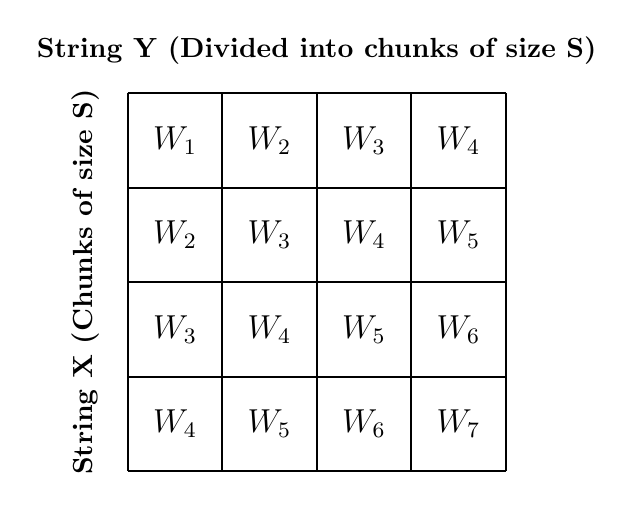
\begin{tikzpicture}[scale=1.2]
        % Draw the grid
        \draw[thick, color=black] (0,0) grid (4,4);
        
        % Fill in the waves
        \foreach \x/\y/\w in {0/3/1, 1/3/2, 0/2/2, 2/3/3, 1/2/3, 0/1/3, 3/3/4, 2/2/4, 1/1/4, 0/0/4, 3/2/5, 2/1/5, 1/0/5, 3/1/6, 2/0/6, 3/0/7} {
            \node at (\x+0.5, \y+0.5) {\large $W_{\w}$};
        }
        
        % Labels
        \node[above, font=\bfseries] at (2,4.2) {String Y (Divided into chunks of size S)};
        \node[rotate=90, above, font=\bfseries] at (-0.2,2) {String X (Chunks of size S)};
    \end{tikzpicture}
    \caption{A $4 \times 4$ Logical Grid showing 7 independent Diagonal Waves ($W_1$ to $W_7$). Tiles with the same wave number can be processed in parallel.}
    \label{fig:wavefront_grid}
\end{figure}

The total number of diagonal waves for a $K \times K$ grid is exactly $2K - 1$. The algorithm iterates through each wave $d$ (where $d$ ranges from 1 to $2K - 1$), assigning the independent tiles to the available processors. 

\subsection{Phase 3: Local Tile Computation (The PRAM-EM Hybrid Phase)}
For a given wave, the independent tiles are distributed among the processors. For each assigned tile, a processor executes three strict steps:

\begin{itemize}
    \item \textbf{Read Phase (I/O):} The processor fetches the $S$-length substring chunks, along with the boundaries from the top and left tiles. Because this is a Concurrent Read (CR) model, adjacent tiles on the same wave can read the same corner boundary simultaneously without queuing.
    
    \item \textbf{Compute Phase (CPU):} The processor calculates the $S \times S$ LCS matrix internally. By isolating the computation inside the fast internal memory, the processor can run the standard sequential DP algorithm at maximum speed. \textit{Zero external I/O occurs during this phase}, meaning the processor never has to pause to wait for the slow disk until the entire tile is completely finished.
    
    \item \textbf{Write Phase (I/O):} The processor extracts only the newly computed bottom row and rightmost column of the tile and writes them back to external memory. Because processors are assigned entirely different tiles, their output boundaries map to different blocks. This perfectly satisfies the Exclusive Write (EW) condition.
\end{itemize}

This strict separation between reading, computing, and writing is what gives the Tiled Wavefront Algorithm its power. By grouping thousands of small calculations into a few large block transfers, the algorithm effectively hides the high latency of the external disk. This ensures that the expensive processors spend their time actively computing answers rather than sitting idle waiting for data.


\begin{algorithm}[H]

    \caption{Tiled Wavefront LCS on the PEM Model}
    \label{alg:tiled_wavefront}
    \begin{algorithmic}[1]
    \Require Strings $X, Y$ of length $N$ in External Memory (EM); $P$ processors; Internal Memory capacity $M$; Block size $B$.
    \Ensure The computed boundaries of the Longest Common Subsequence (LCS) matrix in EM.

\Statex \Comment{\textbf{Phase 1: Initialization}}
\State $S \gets \Theta(\sqrt{M})$ \Comment{Size tile to fit fully in internal memory}
\State $K \gets \lceil N/S \rceil$ \Comment{Logical grid is $K \times K$ tiles}
\For{\textbf{all} $k \gets 1$ \textbf{to} $N$ \textbf{in parallel using} $P$ processors}
    \State $C[k, 0] \gets 0$
    \State $C[0, k] \gets 0$ \Comment{Initialize base cases directly in EM}
\EndFor

\Statex \Comment{\textbf{Phase 2: Wavefront Scheduling}}
\For{$d \gets 1$ \textbf{to} $2K - 1$} \Comment{Iterate over every diagonal wave}
    \State $W_d \gets \{ T(i,j) \mid i + j - 1 = d, \text{ for } 1 \le i, j \le K \}$
    
    \Statex \hspace{0.5cm}\Comment{\textbf{Phase 3: Local Tile Computation}}
    \For{\textbf{each} tile $T(i,j) \in W_d$ \textbf{in parallel using} $P$ processors}
        
        \Statex \hspace{1cm}\Comment{\textit{Step 3a: Concurrent Read (I/O)}}
        \State Read string chunks $X[(i-1)S+1 \dots iS]$ and $Y[(j-1)S+1 \dots jS]$ from EM
        \State Read top boundary from tile $T(i-1, j)$ from EM
        \State Read left boundary from tile $T(i, j-1)$ from EM
        
        \Statex \hspace{1cm}\Comment{\textit{Step 3b: Local Processing (CPU)}}
        \State Compute $S \times S$ LCS matrix for $T(i,j)$ strictly in local internal memory
        
        \Statex \hspace{1cm}\Comment{\textit{Step 3c: Exclusive Write (I/O)}}
        \State Write newly computed bottom boundary of $T(i,j)$ to EM
        \State Write newly computed right boundary of $T(i,j)$ to EM
    \EndFor
\EndFor
        
    \end{algorithmic}
\end{algorithm}



\section{Detailed Numerical Trace}

To clearly illustrate how the Tiled Wavefront Algorithm adapts to limited hardware, we trace its execution using concrete parameters. 

Assume a highly constrained PEM environment where:
\begin{itemize}
    \item Processors ($P$) = 3
    \item Internal Memory ($M$) = 16 words (allowing a tile size of $S = 4$)
    \item Block Size ($B$) = 2 words
\end{itemize}

We are given two strings, $X$ and $Y$, both of length $N=16$. Because $S=4$, the strings are divided into 4 chunks, generating a $4 \times 4$ logical grid containing exactly 16 tiles (as seen in Figure \ref{fig:wavefront_grid}). There are $2(4) - 1 = 7$ waves. Table \ref{tab:processor_schedule} demonstrates the parallel schedule.

\begin{table}[h!]
\centering
\renewcommand{\arraystretch}{1.2}
\begin{tabular}{@{}llccc@{}}
\toprule
\textbf{Wave ($d$)} & \textbf{Active Tiles} & \textbf{Processor 1} & \textbf{Processor 2} & \textbf{Processor 3} \\ \midrule
Wave 1 & $T(1,1)$ & $T(1,1)$ & \textit{Idle} & \textit{Idle} \\
Wave 2 & $T(1,2), T(2,1)$ & $T(1,2)$ & $T(2,1)$ & \textit{Idle} \\
Wave 3 & $T(1,3), T(2,2), T(3,1)$ & $T(1,3)$ & $T(2,2)$ & $T(3,1)$ \\
\midrule
Wave 4 (Round a) & \textit{4 tiles available} & $T(1,4)$ & $T(2,3)$ & $T(3,2)$ \\
Wave 4 (Round b) & & $T(4,1)$ & \textit{Idle} & \textit{Idle} \\
\midrule
Wave 5 & $T(2,4), T(3,3), T(4,2)$ & $T(2,4)$ & $T(3,3)$ & $T(4,2)$ \\
Wave 6 & $T(3,4), T(4,3)$ & $T(3,4)$ & $T(4,3)$ & \textit{Idle} \\
Wave 7 & $T(4,4)$ & $T(4,4)$ & \textit{Idle} & \textit{Idle} \\ \bottomrule
\end{tabular}
\caption{Parallel Processor Schedule. Notice how Wave 4, having more tiles than processors, is automatically divided into two rounds to balance the load.}
\label{tab:processor_schedule}
\end{table}

\subsection{Key Observations from the Trace}
\textbf{1. Massive I/O Savings:} In Wave 1, Processor 1 reads 8 blocks of data and writes 4 blocks. In return, it performs $S^2 = 16$ internal DP calculations. As $M$ scales to realistic sizes (e.g., $M = 1,000,000$ words, $S=1000$), a processor performs one million computations for only a few hundred block transfers, virtually eliminating the I/O bottleneck.

\textbf{2. Automatic Load Balancing:} The algorithm gracefully handles the "bulk" of the matrix. In Wave 4, there are 4 independent tiles but only 3 processors. The schedule automatically breaks this into two rounds (4a and 4b). This mechanism forms the physical basis for Brent's Theorem, which we will use in Chapter 4 to mathematically prove the algorithm's optimal performance.
